% details-of-test-conditions.tex
\chapter{Modelling and Simulation}\label{Appendix:sim}

\section{Propulsion Interpolation Scheme}

\begin{figure}[ht]
	\centering
	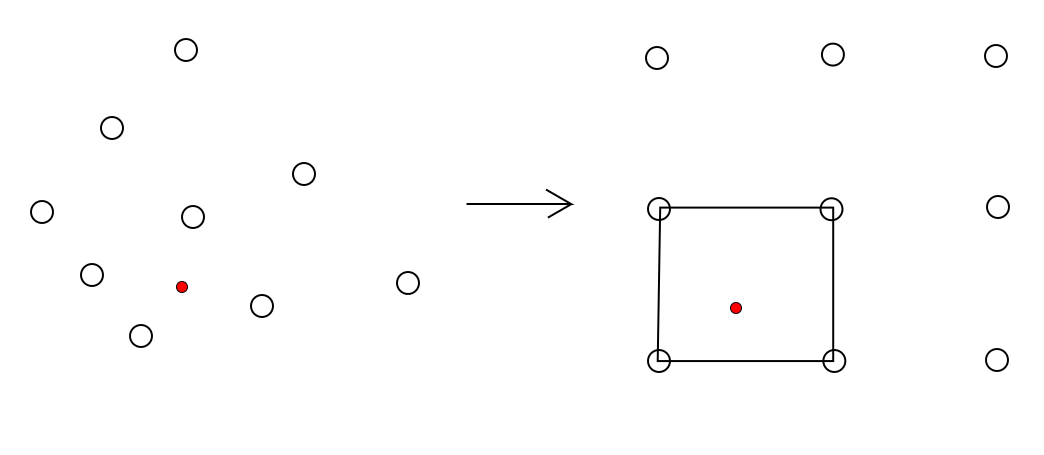
\includegraphics[width=0.8\linewidth]{figures/A1_uncertainty-analysis/interp}
	\caption{The transformation to a normalised interpolation scheme.}
	\label{fig:interp}
\end{figure}
This section describes the interpolation scheme used for the C-RESTM10 database to determine specific impulse.
The C-RESTM10 engine database consists of a set of engine conditions, including specific impulse, ordered by the inlet Mach number and temperature. This data set must be interpolated, to calculate the performance of the engine at each flight condition. However, no inlet Mach number and temperature values are repeated between any of the C-RESTM10 data points. This makes for a scattered data set which complicates the process of interpolating for specific impulse. It was observed that when interpolating for specific impulse, a scattered interpolation produces particularly poor results, and that fitting splines to the data set is the only way to produce an appropriate interpolation scheme. However, even when splines were fit, and the general trends of the specific impulse were matched, minuscule oscillations were still present in the interpolated values. These oscillations do not significantly affect a forward simulation, however, when using the vehicle model as part of an optimal control calculation, they can affect the convergence process. Consequently, it was necessary to craft a bespoke interpolation scheme in order to accurately interpolate the specific impulse of the vehicle. 

This interpolation begins by designating a new coordinate system, normalised to [0 1], running from data point with the lowest inlet temperature [0,0], to the data point with the highest inlet temperature [1,1]. Each data point is then given a set of normalised coordinates, and a cubic spline is fit to this set of normalised points using MATLAB's \textsf{griddedInterpolant} function. The normalised, orderd, data set ensures that this cubic spline is smooth, with no oscillations present. In order to interpolate at a specific location, each data point bounding the interpolation region is set as the corner of a square of data points in normalised coordinates. This is illustrated in Figure \ref{fig:interp}. The distance to each of these bounding data points is calculated, and the location to be interpolated is assigned a set of normalised coordinates. This set of normalised coordinates is used to interpolate for specific impulse. 

This process is accurate, but computationally time consuming, and would increase the computation time of the optimisation process significantly if implemented directly within the vehicle model.
 In order to expedite the interpolation process, interpolations are performed for the specific impulse for every combination of inlet Mach number and temperature present in the C-RESM10 database. This creates a grid of interpolated data points, which includes all of the data points present in the C-RESTM10 database. This grid of interpolated specific impulse values is then used as a new data set, which is now in \textsf{meshgrid} form, by which the specific impulse is interpolated. A bivariate spline is fitted to this grid of data points, using MATLAB's \textsf{griddedInterpolant} function, which is accessed by the vehicle model to determine specific impulse during flight.  







\section{SPARTAN Flow Results}
\begin{figure}[ht]
	\centering
	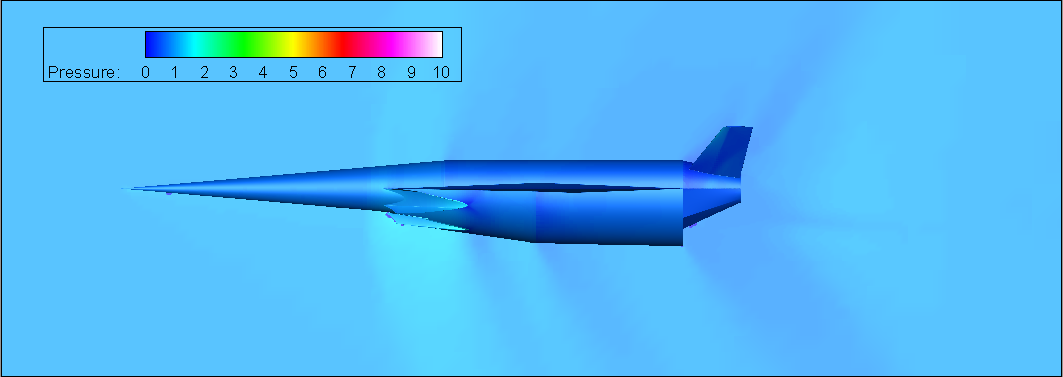
\includegraphics[width=0.9\linewidth]{figures/3_vehicle_design/M1p1AoA6}
	\caption{CART3D flow result for the SPARTAN, at Mach 1.1, 6$^\circ$ angle of attack.}
	\label{fig:M1}
\end{figure}
\begin{figure}[ht]
	\centering
	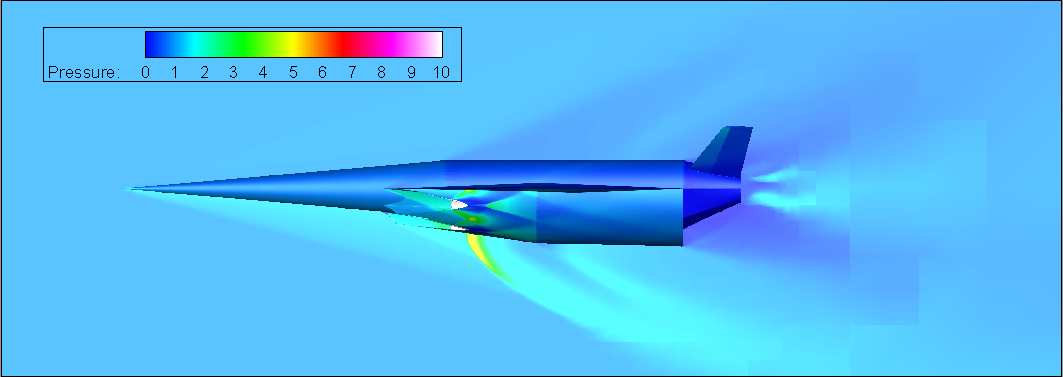
\includegraphics[width=0.9\linewidth]{figures/3_vehicle_design/M3AoA6}
	\caption{CART3D flow result for the SPARTAN, at Mach 3, 6$^\circ$ angle of attack.}
	\label{fig:M3AoA6}
\end{figure}
This section shows additional flow results for the SPARTAN, calculated using Cart3D.
Figures \ref{fig:M1} and \ref{fig:M3AoA6} show flow results for the SPARTAN, at Mach numbers of 1.1 and 3 respectively. It can be observed that at Mach 1.1, the bow shock is not significant, and the shock structure that is evident at higher speeds has not yet formed. At Mach 3, the unstarted C-REST engines are evident, causing significant amounts of the air entering the inlet to be expelled. Shock-shock interaction structures are evident on the cowl of the engines, causing areas of localised high pressure.


\FloatBarrier
\section{Cart3D Mesh}
\begin{figure}[ht]
	\centering
	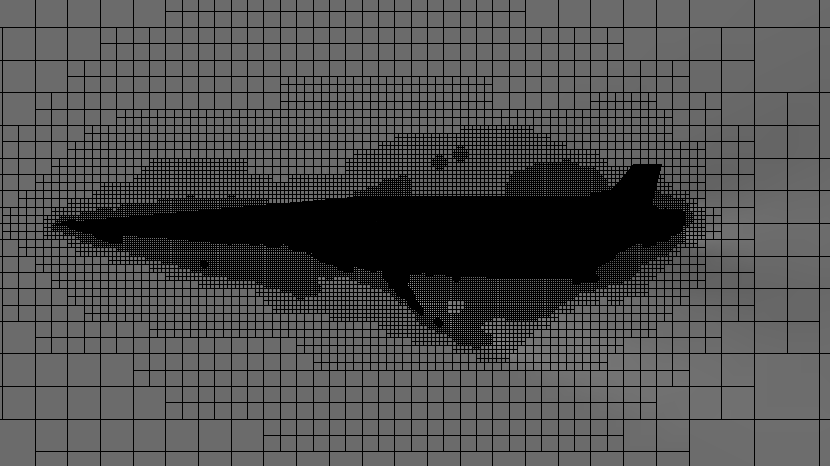
\includegraphics[width=0.7\linewidth]{figures/3_vehicle_design/M3AoA6GRID}
	\caption{Adapted mesh of the SPARTAN at Mach 6 3$^\circ$ angle of attack.}
	\label{fig:M3AoA6GRID}
\end{figure}

\begin{figure}[ht]
	\centering
	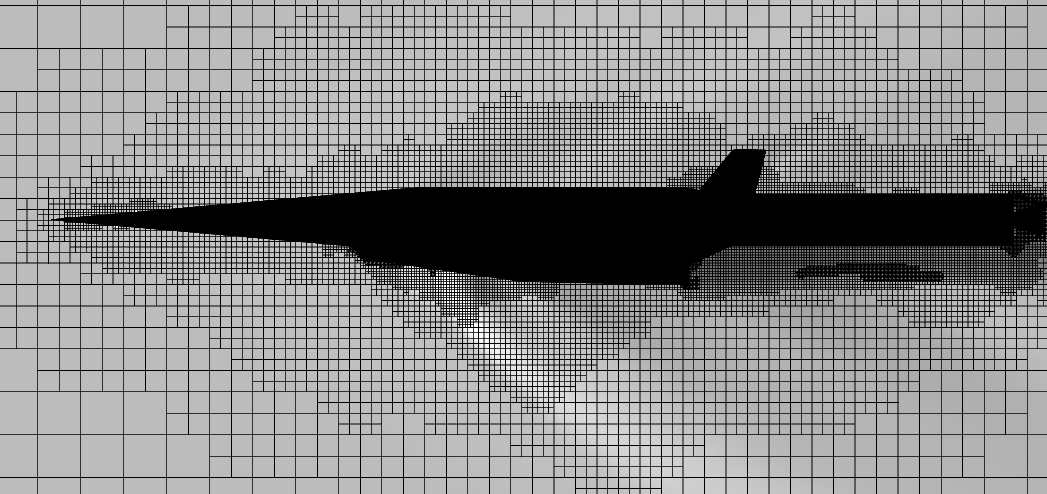
\includegraphics[width=0.7\linewidth]{figures/3_vehicle_design/CARTmesh}
	\caption{Adapted mesh around the SPARTAN and first stage vehicles, flying at Mach 2, -1$^\circ$ angle of attack.}
	\label{fig:CARTmesh}
\end{figure}
This section illustrates the converged meshes used by Cart3D.
Figures \ref{fig:M3AoA6GRID} and \ref{fig:CARTmesh} show adapted meshes for Cart3D solutions of the SPARTAN, and the SPARTAN and first stage. These meshes have been generated adaptively by Cart3D during the solution process. It can be observed that the mesh clusters around the vehicle, particularly in regions where strong shocks are present, where the mesh clusters at the shock front. 



\FloatBarrier
\section{Performance of the SPARTAN During Fly-Back}
Figure \ref{fig:returnIspStandard} shows the performance of the SPARTAN during the boost phase, described in Section \ref{sec:boost}. 

\begin{figure}[ht]
	\centering
	\includegraphics[width=0.7\linewidth]{../LODESTAR_FINAL/Results/mode11/returnIspStandard}
	\caption{The performance of the SPARTAN during the boost phase. Light blue indicates that the scramjet engines are turned on.}
	\label{fig:returnIspStandard}
\end{figure}


\chapter{Example and Verification}

\section{GPOPS-2 Example - Brachistochrone Problem}

This section describes a short example of an optimal control problem solved in GPOPS-II. The purpose of this example is to demonstrate the effectiveness of the pseudospectral method and GPOPS-II, and to provide a simple example case to establish the terminology of an optimal control problem.  


The brachistochrone (from the Greek for 'shortest time') problem is a simple optimal control problem, which describes a ball rolling in two dimensions under gravity. The objective is to find the curve of descent which will minimise the time from point \textit{a}, where the ball is at rest, to point \textit{b}. It is assumed that gravity is constant and that there is no forces other than gravity acting on the ball. 
The analytical solution of this problem can be computed using the Euler-Lagrange equation as the equations describing a cycloid:

$x = A(\theta + \sin\theta) $,

$y=A(1 - \cos\theta)$

This problem is included within GPOPS-2 as an example problem, and has been solved to illustrate the GPOPS-2 solution set-up\cite{Rao2010}. Table \ref{tab:brachistochrone} describes the set-up of the optimal control problem in GPOPS-2. The dynamic equations for the Brachistochrone problem are:

$\dot{x} = v*cos(u)$,

$\dot{y} = v*sin(u)$,

$\dot{v} = g*sin(u)$.

\noindent These equations are provided to GPOPS-2 as the time-variant system model in this form. The control variable is set to be the descent angle. The initial constraints are defined to initiate the ball at rest at the origin, and the terminal constraints are defined to terminate the problem at coordinates of [2,2]. The cost is set to minimum time, so that the solution will be the descent angle which minimises the time to get from the initial position, to the end position. 

\begin{table}
	\centering
	\begin{tabular}{|c|c|}
		\hline Primal Variables  & x Position\\& y Position\\& Velocity\\ 
		\hline Control Variables  & Angle of Descent\\ 
		\hline Initial Constraints  & Velocity\\ & x Position\\ & y Position\\
		\hline Terminal Constraints &  x Position\\ & y Position\\
		\hline Path Constraints & None \\ 
		\hline Target Cost & Minimum Time \\ 
		\hline 
	\end{tabular} 
	\caption{Optimisation setup of the Brachistochrone problem. }
	\label{tab:brachistochrone}
\end{table}


The GPOPS-2 solution to the Brachistochrone problem is shown in Figure \ref{fig:Brachistochrone}, matching the analytical solution almost exactly. This is expected in this case, as the dynamics of the basic Brachistochrone problem are very simple. As the dynamics become more complex, it is no longer possible to obtain an analytical solution.  

\begin{figure}[ht]
	\centering
	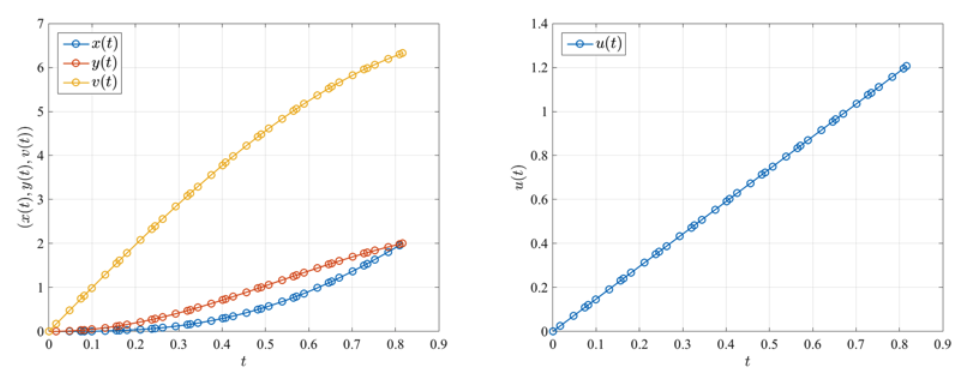
\includegraphics[width=0.9\linewidth]{figures/4_LODESTAR/Brachistochrone}
	\caption{The solution to the Brachistochrone problem, solved in GPOPS-2\cite{Rao2010}.}
	\label{fig:Brachistochrone}
\end{figure}


		
		\section{Optimised Trajectory Analysis}
		
		This section presents an example of the convergence and verification of a trajectory optimised using GPOPS-2, within LODESTAR. The convergence and verification of a maximum payload-to-orbit trajectory solution, with SPARTAN fly-back (Case 11) is shown. 
		
	\subsection{Mesh History}
	
	\begin{figure}[ht]
		\centering
		\includegraphics[width=0.8\linewidth]{../LODESTAR_FINAL/Results/mode11/MeshHistory}
		\caption{The mesh history of each phase of the optimised, maximum payload-to-orbit trajectory with SPARTAN fly-back (Case 11). the phases are shown in each subfigure as follows: a) first stage rocket, b) SPARTAN acceleration, c) SPARTAN fly-back and d) third stage.}
		\label{fig:MeshHistory}*
	\end{figure}
	The mesh history of the optimal trajectory solution is shown in Figure \ref{fig:MeshHistory}. The mesh is updated by GPOPS-2 in each iteration of the optimal solution. It can be observed that the meshes of the first and third stage rockets contain significantly less node points at the final iteration than the meshes of the SPARTAN's acceleration and return. This is due to the relatively simple dynamics and shorter flight time of the first and third stages. The first stage shows a cluster of nodes at the beginning of its trajectory, in the subsonic, transonic and low Mach regimes. In this region, the aerodynamics are changing rapidly, and the nodes are clustered to accurately capture the dynamic behaviour of the vehicle. After transition occurs to supersonic flight, the aerodynamics and engine performance of the vehicle change more slowly, and the nodes become more widely spaced. In contrast, the acceleration of the SPARTAN shows significant node density throughout. The operation of the SPARTAN is complex, as the dynamics of the vehicle and the performance of the scramjet engines vary significantly, even during relatively level flight. For this reason, the nodes of the return flight show even greater density. The trajectory conditions change significantly as the SPARTAN performs skipping manoeuvres, and transitions through the various return phases, necessitating high node density to capture the vehicle dynamics, particularly between powered and unpowered flight. The trajectories of the SPARTAN also last for a significantly longer time than the rocket trajectories, requiring more total nodes to accurately capture the vehicle dynamics. The third stage shows the least nodes at the final mesh iteration, as the dynamics of the third stage are relatively simple. Some node  clustering is observed in the first part of the trajectory, where the atmospheric density is still significant. 
	
		
		
		\subsection{Verification}
		
		After a trajectory has been calculated, it must be verified to ensure that the optimal control solver has converged correctly. Details on this verification are provided in Section \ref{sec:verification}. Figure \ref{fig:HamiltonianStandard} shows the Hamiltonian time history for the optimised trajectory solution of Case 11. For an optimal solution to be found, the Hamiltonian should be equal to 0 at all points over every phase. In a practical solution, a Hamiltonian close to 0 is acceptable, which is observable over all phases in the optimised solution. The Hamiltonian is close to 0 at all points of the trajectory, indicating that an optimal solution has been found. 
		\begin{figure}[ht]
			\centering
			\includegraphics[width=0.9\linewidth]{../LODESTAR_FINAL/Results/mode11/HamiltonianStandard}
			\caption{The Hamiltonian time history of each phase of the maximum payload-to-orbit optimised trajectory, with SPARTAN fly-back (Case 11).}
			\label{fig:HamiltonianStandard}
		\end{figure}
		
		The next step in the verification process is to ensure that the dynamic constraints of the optimal control problem holds across the entire solution, ie. $\dot{\textbf{x}}(t) = f[t,\textbf{x}(t),\textbf{u}(t)]$. This is the most important step in the verification process, which checks that the optimal control solver has converged correctly, so that the physical dynamics of the vehicle are being correctly represented by the polynomial approximations within GPOPS-2. The dynamic constraints are tested by first calculating the dynamics of each vehicle at every node of the solution, using the vehicle simulations. These dynamics are then integrated over time using trapezoidal integration, starting at the initial conditions of each phase. The integrated dynamics are then compared to the states of the optimised solution. If the dynamic constraints have been satisfied, then the integrated dynamics of the system will be equal to the state variables of the solution. The error in the dynamic constraints of each state are shown in Figure \ref{fig:VerificationStandard}, calculated as the difference between the integrated dynamics and each state variable, normalised to the range of the state variable. 
		It can be observed that all errors in the dynamic constraints are very small. The error that is present is likely to be due to the inaccuracies of the trapezoidal method, which is significantly less accurate than the approximating polynomials of the pseudospectral method. 
		
	
		
		\begin{figure}[ht]
			\centering
			\includegraphics[width=0.9\linewidth]{../LODESTAR_FINAL/Results/mode11/VerificationStandard}
			\caption{The error between the integrated dynamics of the system, and the solution states of each phase of the maximum payload-to-orbit optimised trajectory, with SPARTAN fly-back (Case 11). Normalised to the range of each state.}
			\label{fig:VerificationStandard}
		\end{figure}
		
		The final verification step is a forward simulation of each phase. This forward simulation compares the solution state with a simulation which is forward integrated using only the controls of each stage. This is the most stringent method of checking the validity of the solution dynamics. However, it is expected that this verification will have significantly higher errors than the check which verifies the dynamics of each state independently, as the interdependencies of each state come into play, and small errors are compounded. Figure \ref{fig:ForwardErrorStandard} shows the error between the forward simulation and the solution states. As described in Section \ref{sec:verification}, the forward simulation of the return flight is separated into three segments, at 1/6th and 1/3rd of the flight time. The errors in the forward simulation of each stage are observed to be acceptably small, significantly under 1\% in all cases, and it is evident that compounding errors are the cause of the most extreme deviations. 
		
		\begin{figure}[ht]
			\centering
			\includegraphics[width=0.9\linewidth]{../LODESTAR_FINAL/Results/mode11/ForwardErrorStandard}
			\caption{The error between the forward simulated states, and the solution states of each phase of the maximum payload-to-orbit optimised trajectory, with SPARTAN fly-back (Case 11). Normalised to the range of each state.}
			\label{fig:ForwardErrorStandard}
		\end{figure}
		
		\chapter{Alternate Trajectory Cases}
		
		\section{Maximum Payload-To-Orbit Trajectory With Dynamic Pressure Constraint}\label{sec:Appendix_qconst}
		
		The maximum payload-to-orbit trajectory of the launch system with no SPARTAN fly-back (Case 2) was found to involve a significant altitude raising manoeuvre in the middle of the acceleration trajectory of the SPARTAN. Discerning the benefits of this altitude raising manoeuvre proved complex, requiring a trajectory to be calculated in which the altitude raising manoeuvre is prevented from occurring. This section describes an optimised trajectory in which the middle section of the SPARTAN's acceleration is constrained to flight at maximum dynamic pressure. 
		
		 This trajectory was optimised for maximum payload-to-orbit, with a 50kPa dynamic constraint between Mach numbers of 6 and 8, the region in which the altitude raising manoeuvre was observed to occur. This constraint successfully removed the altitude raising manoeuvre from the maximum payload-to-orbit optimised trajectory, allowing for a comparison to be made to quantify the benefits of the altitude raising manoeuvre. This comparison is made in Section \ref{sec:optimisednoreturn}. Figures \ref{fig:FirstStageqConstrained68},  \ref{fig:SecondStageqConstrained68} and \ref{fig:ThirdStageqConstrained68} show the maximum payload-to-orbit trajectory constrained to 50kPa between Mach numbers 6 to 8, and Table \ref{tab:constrained68} details key parameters of the trajectory. 
		
	\begin{table}[ht]
	\centering
\begin{tabular}{l c } 
	\hline \textbf{Trajectory Condition}
	& Value

	\\
	\hline \textbf{Payload to Orbit (kg)}
	& \textbf{\PayloadToOrbitqconstrainedNoReturn}
	\\
	\textbf{Total $\eta_{exergy}$ (\%)}
	& \textbf{\totalExergyEffqconstrainedNoReturn}
	\\
	\hline 
	\textbf{1$^{st}$ Stage $\eta_{exergy}$ (\%)}
	& \textbf{\firstExergyEffqconstrainedNoReturn}
	\\
	\textbf{Separation Alt, 1$\rightarrow$2 (km)}
	& \firstsecondSeparationAltqconstrainedNoReturn
	\\
	\textbf{Separation v, 1$\rightarrow$2 (m/s)}
	& \firstsecondSeparationvqconstrainedNoReturn
	\\
	\textbf{Separation $\gamma$, 1$\rightarrow$2 (deg)}
	& \firstsecondSeparationgammaqconstrainedNoReturn
	\\
	\hline 
	\textbf{2$^{nd}$ Stage $\eta_{exergy}$ (\%)}
	& \textbf{\secondExergyEffqconstrainedNoReturn}
	\\
	\textbf{Separation Alt, 2$\rightarrow$3 (km)}
	& \secondthirdSeparationAltqconstrainedNoReturn
	\\
	\textbf{Separation $v$, 2$\rightarrow$3 (m/s)}
	& \secondthirdSeparationvqconstrainedNoReturn
	\\
	\textbf{Separation $\gamma$, 2$\rightarrow$3 (deg)}
	& \secondthirdSeparationgammaqconstrainedNoReturn
	\\
	\textbf{2$^{nd}$ Stage Flight Time (s)}
	& \secondFlightTimeqconstrainedNoReturn
	\\
	\textbf{2$^{nd}$ Stage Distance Flown (km)}
	& \SecondDistqconstrainedNoReturn
	\\
	\hline 
	\textbf{3$^{rd}$ Stage $\eta_{exergy}$ (\%)}
	& \textbf{\thirddExergyEffqconstrainedNoReturn}
	\\
	\textbf{3$^{rd}$ Stage $t$, $q >$ 5kpa (s)}
	& \thirdqOverFiveqconstrainedNoReturn
	\\
	\textbf{3$^{rd}$ Stage max $\alpha$ (deg)}
	& \thirdmaxAoAqconstrainedNoReturn
	\\
	\textbf{3$^{rd}$ Stage Fuel Mass (kg)}
	& \thirdmFuelqconstrainedNoReturn
	\\
	\hline 
\end{tabular} 
\caption{A summary of key results from the maximum payload-to-orbit trajectory, constrained to 50kPa between Mach numbers 6 to 8.}
\label{tab:constrained68}

	\end{table}
		
\begin{figure}[th]
\centering
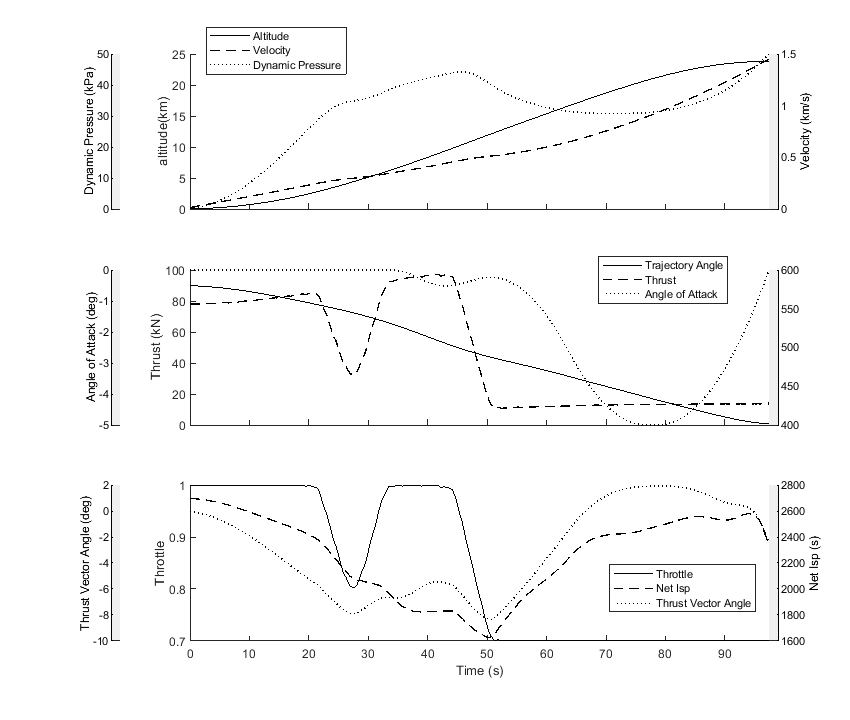
\includegraphics[width=0.9\linewidth]{../LODESTAR_FINAL/Results/10-qconstrained/FirstStageConstq}
\caption{The optimised maximum payload-to-orbit trajectory of the launch system constrained to 50kPa between Mach numbers 6 to 8, under power of the first stage rocket.}
\label{fig:FirstStageqConstrained68}
\end{figure}
		
\begin{figure}[th]
\centering
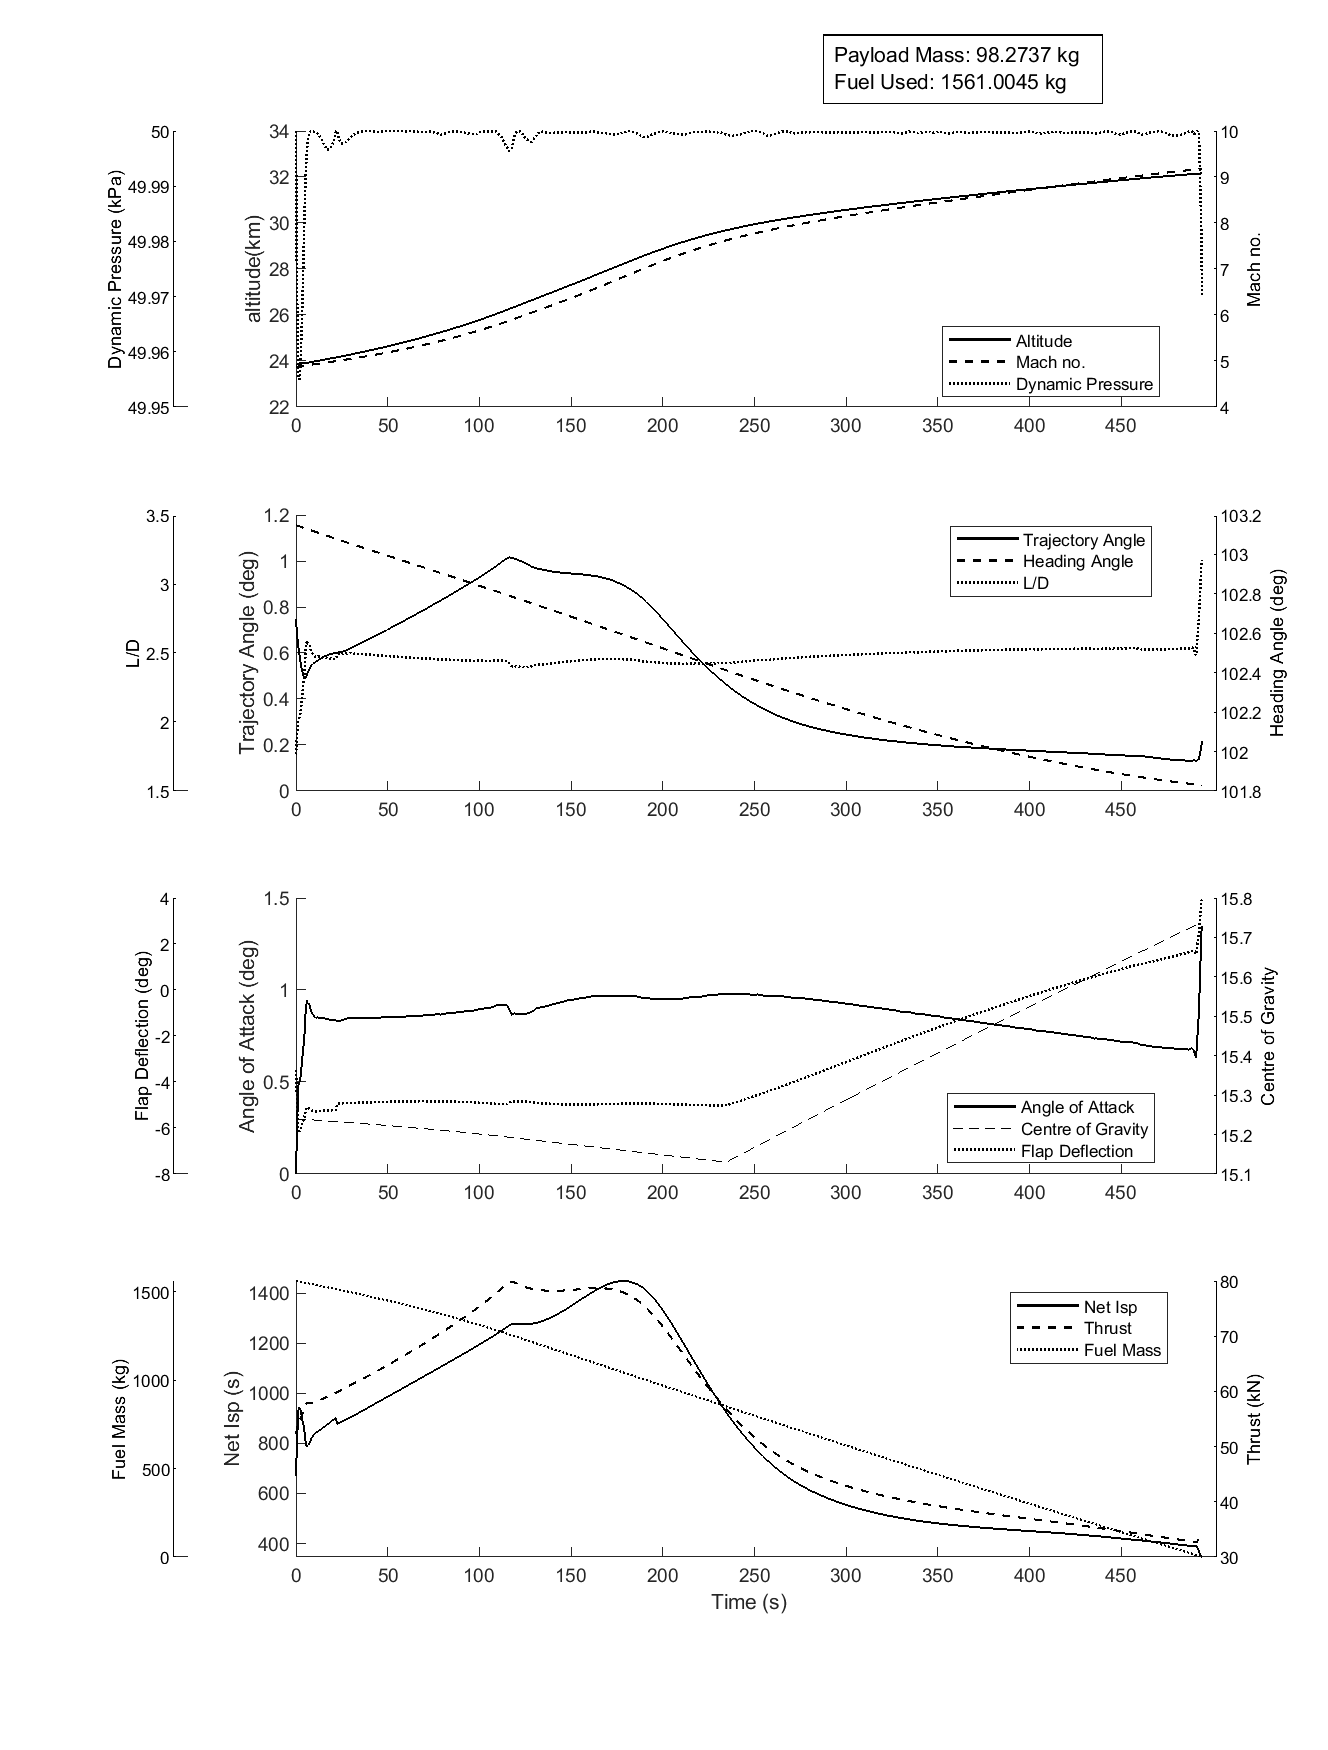
\includegraphics[width=0.9\linewidth]{../LODESTAR_FINAL/Results/10-qconstrained/SecondStageConstq}
\caption{The optimised maximum payload-to-orbit trajectory of the SPARTAN, constrained to 50kPa between Mach numbers 6 to 8.}
\label{fig:SecondStageqConstrained68}
\end{figure}

\begin{figure}[th]
\centering
\includegraphics[width=0.9\linewidth]{../LODESTAR_FINAL/Results/10-qconstrained/ThirdStageConstq}
\caption{The third stage trajectory of the launch system flying the maximum payload-to-orbit trajectory, constrained to 50kPa between Mach numbers 6 to 8.}
\label{fig:ThirdStageqConstrained68}
\end{figure}










\section{Sonic Boom Ground Effects}
\begin{figure}[ht]
	\centering
	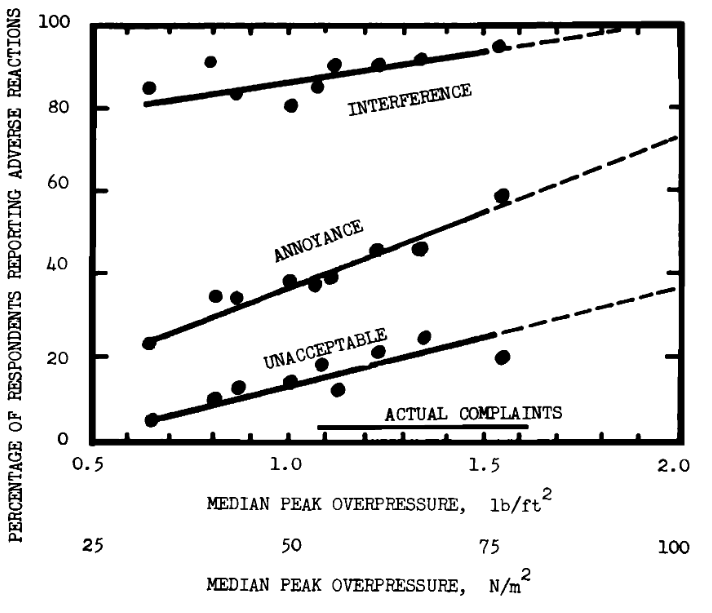
\includegraphics[width=0.6\linewidth]{figures/6_FlyBack/OverPressureResponse}
	\caption{The level of population annoyance with increasing overpressure.}
	\label{fig:OverPressureResponse}
\end{figure}

The flight of a hypersonic vehicle has the potential to create significant overpressures on the ground due to sonic booms. This section describes the effects of the sonic booms generated by the SPARTAN. 

Even when a hypersonic vehicle is flying at high altitudes, the overpressures on the ground may still be large enough to have detrimental effects on any populated areas being overflown. The overpressure from sonic booms can cause significant annoyance to the populace, or in more extreme cases, long term damage to building structures or peoples health. 
When the SPARTAN is launched to a sun synchronous orbit from the Equatorial Launch Australia launch site, it flies over a significant portion of Papua. Fortunately, Papua is sparsely populated, and the number of towns flown over by the SPARTAN will be low. However the effects on these population centres may still be significant. In order to assess the impact of the SPARTAN's flight, the magnitude of the overpressure from its sonic booms must be calculated. 
\begin{figure}[ht]
	\centering
	\includegraphics[width=0.9\linewidth]{../LODESTAR_FINAL/Results/mode11/OverPressureStandard}
	\caption{The sonic boom overpressure on the ground, for the optimised trajectory path (Case 11).}
	\label{fig:OverPressureStandard}
\end{figure}

The sonic boom overpressures are estimated using the 'first cut' estimation technique \cite{Carlson1972}. This estimation technique can approximate sonic boom overpressures moderately well, and is useful as a first approximation to the sonic boom overpressures generated by an aerospace vehicle. The overpressures generated by the SPARTAN are calculated over its trajectory, shown in Figure \ref{fig:OverPressureStandard}. It is found that overpressures of up to 375.3Pa occur during flight over land during the maximum payload-to-orbit trajectory of the SPARTAN. These overpressures have a low but significant probability of causing cosmetic damage to structures (~1.5\% for plaster and ~0.4\% for glass)\cite{Hershey1976}. In addition, overpressures of these magnitudes have been rated as unacceptably annoying to the majority populace being overflown, as shown in Figure \ref{fig:OverPressureResponse}. 
These overpressures indicate that overflight of populated areas may not be reasonable for the SPARTAN flying its maximum payload-to-orbit trajectory path, with fly-back (Case 11). 


%http://www.dtic.mil/dtic/tr/fulltext/u2/a028512.pdf





\section{Alternate Launch Location}

In this section, an alternate southerly launch is investigated for the rocket-scramjet-rocket launch system, in the case that flight over Papua is not possible. This launch occurs from Streaky Bay, the possible location of a launch site being developed by Southern Launch Australia\cite{Council2016}. The maximum payload-to-orbit has been calculated from this launch site using LODESTAR. Figure \ref{fig:GroundTrackAlternate} shows the ground track of this optimised trajectory, and Table \ref{tab:summaryalternate} details a summary of the key trajectory parameters. The shape of this optimised trajectory is very similar to the optimal trajectory of the launch system launched from the Northern Territory (Case 11). The first stage initially pitches towards the west, separating the SPARTAN in a westerly direction. The SPARTAN then performs a banking manoeuvre to the south, and a pull-up before third stage release. After separation, the SPARTAN exhibits initial turn, boost-skip and approach phases during fly-back, with the scramjet engine igniting three times at the troughs of the first three skips, in the same manner as when launching northerly. A higher payload to orbit is achieved when launching from a southerly location, attaining a total of \PayloadToOrbitAlternate kg of payload-to-orbit, an increase of +2.9\% compared to northerly launch. This payload increase is caused by the rotation of the Earth hindering, rather than assisting, when launching into a retrograde orbit, making launch from a more southerly point desirable. 


\begin{figure}[th]
	\centering
	\includegraphics[width=1\linewidth]{../LODESTAR_FINAL/Results/mode01/GroundTrackAlternate}
	\caption{The optimised maximum payload-to-orbit trajectory of the launch system launching onto a southerly orbit, from Streaky Bay.}
	\label{fig:GroundTrackAlternate}
\end{figure}

\begin{table}
	\centering
	\begin{tabular}{l c} 
		\hline \textbf{Trajectory Condition}
		& Value

		\\
		\hline \textbf{Payload to Orbit (kg)}
		& \textbf{\PayloadToOrbitAlternate}
		\\
		\textbf{Total $\eta_{exergy}$ (\%)}
		& \textbf{\totalExergyEffAlternate}
		\\
		\hline 
		\textbf{1$^{st}$ Stage $\eta_{exergy}$ (\%)}
		& \textbf{\firstExergyEffAlternate}
		\\
		\textbf{Separation Alt, 1$\rightarrow$2 (km)}
		& \firstsecondSeparationAltAlternate
		\\
		\textbf{Separation v, 1$\rightarrow$2 (m/s)}
		& \firstsecondSeparationvAlternate
		\\
		\textbf{Separation $\gamma$, 1$\rightarrow$2 (deg)}
		& \firstsecondSeparationgammaAlternate
		\\
		\hline 
		\textbf{2$^{nd}$ Stage $\eta_{exergy}$ (\%)}
		& \textbf{\secondExergyEffAlternate}
		\\
		\textbf{Separation Alt, 2$\rightarrow$3 (km)}
		& \secondthirdSeparationAltAlternate
		\\
		\textbf{Separation $v$, 2$\rightarrow$3 (m/s)}
		& \secondthirdSeparationvAlternate
		\\
		\textbf{Separation $\gamma$, 2$\rightarrow$3 (deg)}
		& \secondthirdSeparationgammaAlternate
		\\
		\textbf{2$^{nd}$ Stage Flight Time (s)}
		& \secondFlightTimeAlternate
		\\
		\textbf{2$^{nd}$ Stage Distance Flown (km)}
		& \SecondDistAlternate
		\\
		\textbf{2$^{nd}$ Stage Return Fuel (kg)}
		& \returnFuelAlternate
		\\
		\textbf{2$^{nd}$ Stage Return Distance (km)}
		& \returnDistAlternate
		\\
		\hline 
		\textbf{3$^{rd}$ Stage $\eta_{exergy}$ (\%)}
		& \textbf{\thirddExergyEffAlternate}
		\\
		\textbf{3$^{rd}$ Stage $t$, $q >$ 5kpa (s)}
		& \thirdqOverFiveAlternate
		\\
		\textbf{3$^{rd}$ Stage max $\alpha$ (deg)}
		& \thirdmaxAoAAlternate
		\\
		\textbf{3$^{rd}$ Stage Fuel Mass (kg)}
		& \thirdmFuelAlternate
		\\
		\hline 
	\end{tabular} 
	\caption{A summary of key trajectory parameters of the maximum payload-to-orbit trajectory launched in a southerly direction.}
	\label{tab:summaryalternate}
\end{table}




		
		\chapter{Trajectory Plot Comparisons}\label{sec:Appendix_trajectorycomparisons}
		
This section contains trajectory plot comparisons for the sensitivity studies performed in Section \ref{sec:sensitivityNoReturn} and \ref{sec:sensitivity}. Comparisons and analyses between these trajectories are performed in the relevant sections. 
		\clearpage
		\section{Optimised Ascent Trajectory Comparisons With No Fly-Back}
		
		\subsection{Case 3: Maximum Dynamic Pressure Sensitivity Comparison}\label{sec:app_comparison20}
		
		
\begin{figure}[!ht]
\centering
\includegraphics[width=1\linewidth]{../LODESTAR_FINAL/Results/mode20/SecondStageComparison}
\caption{Comparison of SPARTAN ascent trajectories with variation in the maximum dynamic pressure of the SPARTAN.}
\label{fig:SecondStageComparison1}
\end{figure}

\begin{figure}[!th]
\centering
\includegraphics[width=1\linewidth]{../LODESTAR_FINAL/Results/mode20/ThirdStageComparison}
\caption{Comparison of third stage rocket ascent trajectories with variation in the maximum dynamic pressure of the SPARTAN.}
\label{fig:ThirdStageComparison1}
\end{figure}
\FloatBarrier

\clearpage

\subsection{Case 4: SPARTAN Drag Sensitivity Comparison}\label{sec:app_comparison40}

\begin{figure}[!th]
\centering
\includegraphics[width=1\linewidth]{../LODESTAR_FINAL/Results/mode40/SecondStageComparison}
\caption{Comparison of SPARTAN ascent trajectories with variation in the drag of the SPARTAN.}
\label{fig:SecondStageComparison3}
\end{figure}

\begin{figure}[!th]
\centering
\includegraphics[width=1\linewidth]{../LODESTAR_FINAL/Results/mode40/ThirdStageComparison}
\caption{Comparison of third stage rocket ascent trajectories with variation in the drag of the SPARTAN.}
\label{fig:ThirdStageComparison3}
\end{figure}
\FloatBarrier
\clearpage
\subsection{Case 5: SPARTAN Specific Impulse Sensitivity Comparison}\label{sec:app_comparison30}


\begin{figure}[!th]
	\centering
	\includegraphics[width=1\linewidth]{../LODESTAR_FINAL/Results/mode30/SecondStageComparison}
	\caption{Comparison of SPARTAN ascent trajectories with variation in the specific impulse of the SPARTAN.}
	\label{fig:SecondStageComparison2}
	
\end{figure}
\begin{figure}[!th]
	\centering
	\includegraphics[width=1\linewidth]{../LODESTAR_FINAL/Results/mode30/ThirdStageComparison}
	\caption{Comparison of third stage rocket ascent trajectories with variation in the specific impulse of the SPARTAN.}
	\label{fig:ThirdStageComparison2}
\end{figure}
\FloatBarrier
\clearpage
\subsection{Case 6: SPARTAN Mass Sensitivity Comparison}\label{sec:app_comparison100}

\begin{figure}[!th]
\centering
\includegraphics[width=1\linewidth]{../LODESTAR_FINAL/Results/mode100/SecondStageComparison}
\caption{Comparison of SPARTAN ascent trajectories with variation in the mass of the SPARTAN.}
\label{fig:SecondStageComparison4}
\end{figure}

\begin{figure}[!th]
\centering
\includegraphics[width=1\linewidth]{../LODESTAR_FINAL/Results/mode100/ThirdStageComparison}
\caption{Comparison of third stage rocket ascent trajectories with variation in the mass of the SPARTAN.}
\label{fig:ThirdStageComparison4}
\end{figure}
\FloatBarrier
\clearpage
\subsection{Case 7: SPARTAN Fuel Mass Sensitivity Comparison}\label{sec:app_comparison110}
\begin{figure}[!th]
\centering
\includegraphics[width=1\linewidth]{../LODESTAR_FINAL/Results/mode110/SecondStageComparison}
\caption{Comparison of SPARTAN ascent trajectories with variation in the fuel mass of the SPARTAN.}
\label{fig:SecondStageComparison5}
\end{figure}

\begin{figure}[!th]
\centering
\includegraphics[width=1\linewidth]{../LODESTAR_FINAL/Results/mode110/ThirdStageComparison}
\caption{Comparison of third stage rocket ascent trajectories with variation in the fuel mass of the SPARTAN.}
\label{fig:ThirdStageComparison5}
\end{figure}
\FloatBarrier
\clearpage
\subsection{Case 8: Third Stage Mass Sensitivity Comparison}\label{sec:app_comparison80}

\begin{figure}[!th]
\centering
\includegraphics[width=1\linewidth]{../LODESTAR_FINAL/Results/mode80/SecondStageComparison}
\caption{Comparison of SPARTAN ascent trajectories with variation in the mass of the third stage.}
\label{fig:SecondStageComparison6}
\end{figure}


\begin{figure}[!th]
\centering
\includegraphics[width=1\linewidth]{../LODESTAR_FINAL/Results/mode80/ThirdStageComparison}
\caption{Comparison of third stage rocket ascent trajectories with variation in the mass of the third stage.}
\label{fig:ThirdStageComparison6}
\end{figure}

\FloatBarrier
\clearpage
\subsection{Case 9: Third Stage Specific Impulse Sensitivity Comparison}\label{sec:app_comparison90}

\begin{figure}[!th]
	\centering
	\includegraphics[width=1\linewidth]{../LODESTAR_FINAL/Results/mode90/SecondStageComparison}
	\caption{Comparison of SPARTAN ascent trajectories with variation in the specific impulse of the third stage.}
	\label{fig:SecondStageComparison7}
\end{figure}

\begin{figure}[!th]
\centering
\includegraphics[width=1\linewidth]{../LODESTAR_FINAL/Results/mode90/ThirdStageComparison}
\caption{Comparison of third stage rocket ascent trajectories with variation in the specific impulse of the third stage.}
\label{fig:ThirdStageComparison7}
\end{figure}
\FloatBarrier
\clearpage
\subsection{Case 10:Third Stage Drag Sensitivity Comparison}\label{sec:app_comparison70}

\begin{figure}[!th]
\centering
\includegraphics[width=1\linewidth]{../LODESTAR_FINAL/Results/mode70/SecondStageComparison}
\caption{Comparison of SPARTAN ascent trajectories with variation in the drag of the third stage.}
\label{fig:SecondStageComparison8}
\end{figure}


\begin{figure}[!th]
\centering
\includegraphics[width=1\linewidth]{../LODESTAR_FINAL/Results/mode70/ThirdStageComparison}
\caption{Comparison of third stage rocket ascent trajectories with variation in the drag of the third stage.}
\label{fig:ThirdStageComparison8}
\end{figure}

\FloatBarrier
\clearpage
\section{Optimised Ascent Trajectory Comparisons With Fly-Back}
\FloatBarrier
\subsection{Case 12: Dynamic Pressure Sensitivity Comparison}\label{sec:app_comparison21}
\begin{figure}[!th]
\centering
\includegraphics[width=1\linewidth]{../LODESTAR_FINAL/Results/mode21/SecondStageComparison}
\caption{Comparison of SPARTAN ascent trajectories with variation in the maximum dynamic pressure of the SPARTAN.}
\label{fig:SecondStageComparison9}
\end{figure}

\begin{figure}[!th]
\centering
\includegraphics[width=1\linewidth]{../LODESTAR_FINAL/Results/mode21/ThirdStageComparison}
\caption{Comparison of third stage rocket ascent trajectories with variation in the maximum dynamic pressure of the SPARTAN.}
\label{fig:ThirdStageComparison9}
\end{figure}

\begin{figure}[!th]
\centering
\includegraphics[width=1\linewidth]{../LODESTAR_FINAL/Results/mode21/ReturnComparison}
\caption{Comparison of SPARTAN return trajectories with variation in the maximum dynamic pressure of the SPARTAN.}
\label{fig:ReturnComparison}
\end{figure}



\FloatBarrier
\clearpage
\subsection{Case 13: SPARTAN Drag Sensitivity Comparison}\label{sec:app_comparison41}
\begin{figure}[!th]
\centering
\includegraphics[width=1\linewidth]{../LODESTAR_FINAL/Results/mode41/SecondStageComparison}
\caption{Comparison of SPARTAN ascent trajectories with variation in the drag of the SPARTAN.}
\label{fig:SecondStageComparison11}
\end{figure}

\begin{figure}[!th]
\centering
\includegraphics[width=1\linewidth]{../LODESTAR_FINAL/Results/mode41/ThirdStageComparison}
\caption{Comparison of third stage rocket ascent trajectories with variation in the drag of the SPARTAN.}
\label{fig:ThirdStageComparison11}
\end{figure}

\begin{figure}[!th]
\centering
\includegraphics[width=1\linewidth]{../LODESTAR_FINAL/Results/mode41/ReturnComparison}
\caption{Comparison of SPARTAN return trajectories with variation in the drag of the SPARTAN.}
\label{fig:ReturnComparison11}
\end{figure}

\FloatBarrier
\clearpage
\subsection{Case 14:SPARTAN Specific Impulse Sensitivity Comparison}\label{sec:app_comparison31}
\begin{figure}[!th]
	\centering
	\includegraphics[width=1\linewidth]{../LODESTAR_FINAL/Results/mode31/SecondStageComparison}
	\caption{Comparison of SPARTAN ascent trajectories with variation in the specific impulse of the SPARTAN.}
	\label{fig:SecondStageComparison10}
\end{figure}

\begin{figure}[!th]
	\centering
	\includegraphics[width=1\linewidth]{../LODESTAR_FINAL/Results/mode31/ThirdStageComparison}
	\caption{Comparison of third stage rocket ascent trajectories with variation in the specific impulse of the SPARTAN.}
	\label{fig:ThirdStageComparison10}
\end{figure}

\begin{figure}[!th]
	\centering
	\includegraphics[width=1\linewidth]{../LODESTAR_FINAL/Results/mode31/ReturnComparison}
	\caption{Comparison of SPARTAN return trajectories with variation in the specific impulse of the SPARTAN.}
	\label{fig:ReturnComparison10}
\end{figure}
\FloatBarrier
\clearpage
\subsection{Case 15: SPARTAN Mass Sensitivity Comparison}\label{sec:app_comparison101}

\begin{figure}[!th]
\centering
\includegraphics[width=1\linewidth]{../LODESTAR_FINAL/Results/mode101/SecondStageComparison}
\caption{Comparison of SPARTAN ascent trajectories with variation in the mass of the SPARTAN.}
\label{fig:SecondStageComparison12}
\end{figure}

\begin{figure}[!th]
\centering
\includegraphics[width=1\linewidth]{../LODESTAR_FINAL/Results/mode101/ThirdStageComparison}
\caption{Comparison of third stage rocket ascent trajectories with variation in the mass of the SPARTAN.}
\label{fig:ThirdStageComparison12}
\end{figure}

\begin{figure}[!th]
\centering
\includegraphics[width=1\linewidth]{../LODESTAR_FINAL/Results/mode101/ReturnComparison}
\caption{Comparison of SPARTAN return trajectories with variation in the mass of the SPARTAN.}
\label{fig:ReturnComparison12}
\end{figure}

\FloatBarrier
\clearpage
\subsection{Case 16: SPARTAN Fuel Mass Sensitivity Comparison}\label{sec:app_comparison111}

\begin{figure}[!th]
\centering
\includegraphics[width=1\linewidth]{../LODESTAR_FINAL/Results/mode111/SecondStageComparison}
\caption{Comparison of SPARTAN ascent trajectories with variation in the fuel mass of the SPARTAN.}
\label{fig:SecondStageComparison13}
\end{figure}

\begin{figure}[!th]
\centering
\includegraphics[width=1\linewidth]{../LODESTAR_FINAL/Results/mode111/ThirdStageComparison}
\caption{Comparison of third stage rocket ascent trajectories with variation in the fuel mass of the SPARTAN.}
\label{fig:ThirdStageComparison13}
\end{figure}

\begin{figure}[!th]
\centering
\includegraphics[width=1\linewidth]{../LODESTAR_FINAL/Results/mode111/ReturnComparison}
\caption{Comparison of SPARTAN return trajectories with variation in the fuel mass of the SPARTAN.}
\label{fig:ReturnComparison13}
\end{figure}


\FloatBarrier
\clearpage
\subsection{Case 17: Third Stage Mass Sensitivity Comparison}\label{sec:app_comparison81}
\begin{figure}[!th]
\centering
\includegraphics[width=1\linewidth]{../LODESTAR_FINAL/Results/mode81/SecondStageComparison}
\caption{Comparison of SPARTAN ascent trajectories with variation in the mass of the third stage.}
\label{fig:SecondStageComparison14}
\end{figure}

\begin{figure}[!th]
\centering
\includegraphics[width=1\linewidth]{../LODESTAR_FINAL/Results/mode81/ThirdStageComparison}
\caption{Comparison of third stage rocket ascent trajectories with variation in the mass of the third stage.}
\label{fig:ThirdStageComparison14}
\end{figure}



\begin{figure}[!th]
	\centering
	\includegraphics[width=1\linewidth]{../LODESTAR_FINAL/Results/mode81/ReturnComparison}
	\caption{Comparison of SPARTAN return trajectories with variation in the mass of the third stage.}
	\label{fig:ReturnComparison14}
\end{figure}
\FloatBarrier
\clearpage
\subsection{Case 18: Third Stage Specific Impulse Sensitivity Comparison}\label{sec:app_comparison91}

\begin{figure}[!th]
\centering
\includegraphics[width=1\linewidth]{../LODESTAR_FINAL/Results/mode91/SecondStageComparison}
\caption{Comparison of SPARTAN ascent trajectories with variation in the specific impulse of the third stage.}
\label{fig:SecondStageComparison15}
\end{figure}


\begin{figure}[!th]
\centering
\includegraphics[width=1\linewidth]{../LODESTAR_FINAL/Results/mode91/ThirdStageComparison}
\caption{Comparison of third stage rocket ascent trajectories with variation in the specific impulse of the third stage.}
\label{fig:ThirdStageComparison15}
\end{figure}


\begin{figure}[!th]
\centering
\includegraphics[width=1\linewidth]{../LODESTAR_FINAL/Results/mode91/ReturnComparison}
\caption{Comparison of SPARTAN return trajectories with variation in the specific impulse of the third stage.}
\label{fig:ReturnComparison15}
\end{figure}


\chapter{Viscous Drag Variation}

This section presents the sensitivity of the launch system performance to variations in the viscous drag of the SPARTAN. This sensitivity analysis is intended as a reference, to indicate the magnitude of variations in the viscous drag of the SPARTAN due to variations in modelling methods, and is unlikely to be indicative of any physical design variations.
The viscous drag component of the SPARTAN's aerodynamics is calculated using flat plate correlations, which require an estimation of the laminar to turbulent transition point on the body of the SPARTAN\cite{Ward2018}. This transition point is difficult to estimate to a high degree of accuracy, and can have a significant effect on the viscous drag of an aircraft\cite{Ward2018}.
The viscous drag component of the SPARTAN's aerodynamics is varied, in order to assess the impact of the viscous drag model used. Optimal trajectories are calculated with the viscous drag set at levels of 20\%, 50\%, 107\% and 115\% of the baseline, which correspond to the possible viscous drag range due to transition point variation. Table \ref{tab:viscous} details key trajectory parameters of the optimised trajectories, and Figures \ref{fig:SecondStageComparison-}, \ref{fig:ThirdStageComparison-} and \ref{fig:ReturnComparison-} show comparison plots of the optimised trajectories. The sensitivity of the launch system to the viscous drag of the SPARTAN is shown to be relatively low, as the deviations in the viscous drag model are expected to be small, relative to the range tested. This low sensitivity indicating that the modelling process of the viscous drag is unlikely to have a large effect on the accuracy of the maximum payload-to-orbit solution.

\begin{table}[ht]
	\centering
	\begin{tabular}{l c c c c c c} 
		\hline \textbf{Trajectory Condition} \qquad vC$_D$:
		&20\%
		&50\%
		&100\%
		&107\%
		&115\%
		& $\Delta/\Delta$\%vC$_D$
		\\
		\hline \textbf{Payload to Orbit (kg)}
		& \textbf{\PayloadToOrbitvCdTwenty}
		& \textbf{\PayloadToOrbitvCdFifty}
		& \textbf{\PayloadToOrbitvCdStandard}
		& \textbf{\PayloadToOrbitvCdOneHundredSeven}
		& \textbf{\PayloadToOrbitvCdOneHundredFifteen}
		&\textbf{-2.5}
		\\
		\textbf{Payload Variation (\%)}
		& \PayloadVarvCdTwenty
		& \PayloadVarvCdFifty
		& \PayloadVarvCdStandard
		& \PayloadVarvCdOneHundredSeven
		& \PayloadVarvCdOneHundredFifteen
		&-0.31
		\\
		\textbf{Total $\eta_{exergy}$ (\%)}
		& \textbf{\totalExergyEffvCdTwenty}
		& \textbf{\totalExergyEffvCdFifty}
		& \textbf{\totalExergyEffvCdStandard}
		& \textbf{\totalExergyEffvCdOneHundredSeven}
		& \textbf{\totalExergyEffvCdOneHundredFifteen}
		& \textbf{-0.00024}
		\\
		\hline 
		\textbf{1$^{st}$ Stage $\eta_{exergy}$ (\%)}
		& \textbf{\firstExergyEffvCdTwenty}
		& \textbf{\firstExergyEffvCdFifty}
		& \textbf{\firstExergyEffvCdStandard}
		& \textbf{\firstExergyEffvCdOneHundredSeven}
		& \textbf{\firstExergyEffvCdOneHundredFifteen}
		& -
		\\
		\textbf{Separation Alt, 1$\rightarrow$2 (km)}
		& \firstsecondSeparationAltvCdTwenty
		& \firstsecondSeparationAltvCdFifty
		& \firstsecondSeparationAltvCdStandard
		& \firstsecondSeparationAltvCdOneHundredSeven
		& \firstsecondSeparationAltvCdOneHundredFifteen
		& -
		\\
		\textbf{Separation v, 1$\rightarrow$2 (m/s)}
		& \firstsecondSeparationvvCdTwenty
		& \firstsecondSeparationvvCdFifty
		& \firstsecondSeparationvvCdStandard
		& \firstsecondSeparationvvCdOneHundredSeven
		& \firstsecondSeparationvvCdOneHundredFifteen
		& -
		\\
		\textbf{Separation $\gamma$, 1$\rightarrow$2 (deg)}
		& \firstsecondSeparationgammavCdTwenty
		& \firstsecondSeparationgammavCdFifty
		& \firstsecondSeparationgammavCdStandard
		& \firstsecondSeparationgammavCdOneHundredSeven
		& \firstsecondSeparationgammavCdOneHundredFifteen
		& -
		\\
		\hline 
		\textbf{2$^{nd}$ Stage $\eta_{exergy}$ (\%)}
		& \textbf{\secondExergyEffvCdTwenty}
		& \textbf{\secondExergyEffvCdFifty}
		& \textbf{\secondExergyEffvCdStandard}
		& \textbf{\secondExergyEffvCdOneHundredSeven}
		& \textbf{\secondExergyEffvCdOneHundredFifteen}
		& \textbf{-0.064}
		\\
		\textbf{Separation Alt, 2$\rightarrow$3 (km)}
		& \secondthirdSeparationAltvCdTwenty
		& \secondthirdSeparationAltvCdFifty
		& \secondthirdSeparationAltvCdStandard
		& \secondthirdSeparationAltvCdOneHundredSeven
		& \secondthirdSeparationAltvCdOneHundredFifteen
		& -
		\\
		\textbf{Separation $v$, 2$\rightarrow$3 (m/s)}
		& \secondthirdSeparationvvCdTwenty
		& \secondthirdSeparationvvCdFifty
		& \secondthirdSeparationvvCdStandard
		& \secondthirdSeparationvvCdOneHundredSeven
		& \secondthirdSeparationvvCdOneHundredFifteen
		&-33.84
		\\
		\textbf{Separation $\gamma$, 2$\rightarrow$3 (deg)}
		& \secondthirdSeparationgammavCdTwenty
		& \secondthirdSeparationgammavCdFifty
		& \secondthirdSeparationgammavCdStandard
		& \secondthirdSeparationgammavCdOneHundredSeven
		& \secondthirdSeparationgammavCdOneHundredFifteen
		&-0.1
		\\
		\textbf{2$^{nd}$ Stage Flight Time (s)}
		& \secondFlightTimevCdTwenty
		& \secondFlightTimevCdFifty
		& \secondFlightTimevCdStandard
		& \secondFlightTimevCdOneHundredSeven
		& \secondFlightTimevCdOneHundredFifteen
		& -
		\\
		\textbf{2$^{nd}$ Stage Distance Flown (km)}
		& \SecondDistvCdTwenty
		& \SecondDistvCdFifty
		& \SecondDistvCdStandard
		& \SecondDistvCdOneHundredSeven
		& \SecondDistvCdOneHundredFifteen
		& -
		\\
		\textbf{2$^{nd}$ Stage Return Fuel (kg)}
		& \returnFuelvCdTwenty
		& \returnFuelvCdFifty
		& \returnFuelvCdStandard
		& \returnFuelvCdOneHundredSeven
		& \returnFuelvCdOneHundredFifteen
		& -
		\\
		\textbf{2$^{nd}$ Stage Return Distance (km)}
		& \returnDistvCdTwenty
		& \returnDistvCdFifty
		& \returnDistvCdStandard
		& \returnDistvCdOneHundredSeven
		& \returnDistvCdOneHundredFifteen
		&-21.35
		\\
		\hline 
		\textbf{3$^{rd}$ Stage $\eta_{exergy}$ (\%)}
		& \textbf{\thirddExergyEffvCdTwenty}
		& \textbf{\thirddExergyEffvCdFifty}
		& \textbf{\thirddExergyEffvCdStandard}
		& \textbf{\thirddExergyEffvCdOneHundredSeven}
		& \textbf{\thirddExergyEffvCdOneHundredFifteen}
		& \textbf{-0.249}
		\\
		\textbf{3$^{rd}$ Stage $t$, $q >$ 5kpa (s)}
		& \thirdqOverFivevCdTwenty
		& \thirdqOverFivevCdFifty
		& \thirdqOverFivevCdStandard
		& \thirdqOverFivevCdOneHundredSeven
		& \thirdqOverFivevCdOneHundredFifteen
		&-0.24
		\\
		\textbf{3$^{rd}$ Stage max $\alpha$ (deg)}
		& \thirdmaxAoAvCdTwenty
		& \thirdmaxAoAvCdFifty
		& \thirdmaxAoAvCdStandard
		& \thirdmaxAoAvCdOneHundredSeven
		& \thirdmaxAoAvCdOneHundredFifteen
		& -
		\\
		\textbf{3$^{rd}$ Stage Fuel Mass (kg)}
		& \thirdmFuelvCdTwenty
		& \thirdmFuelvCdFifty
		& \thirdmFuelvCdStandard
		& \thirdmFuelvCdOneHundredSeven
		& \thirdmFuelvCdOneHundredFifteen
		&-32.96
		\\
		\hline 
	\end{tabular} 
	\caption{Summary of key trajectory parameters with SPARTAN viscous drag variation.}
	\label{tab:viscous}
\end{table} 


\begin{figure}[!th]
\centering
\includegraphics[width=1\linewidth]{../LODESTAR_FINAL/Results/mode51/SecondStageComparison}
\caption{Comparison of SPARTAN ascent trajectories with variation in the viscous drag of the SPARTAN.}
\label{fig:SecondStageComparison-}
\end{figure}
\begin{figure}[!th]
\centering
\includegraphics[width=1\linewidth]{../LODESTAR_FINAL/Results/mode51/ThirdStageComparison}
\caption{Comparison of third stage ascent trajectories with variation in the viscous drag of the SPARTAN.}
\label{fig:ThirdStageComparison-}
\end{figure}


\begin{figure}[!th]
	\centering
	\includegraphics[width=1\linewidth]{../LODESTAR_FINAL/Results/mode51/ReturnComparison}
	\caption{Comparison of SPARTAN return trajectories with variation in the viscous drag of the SPARTAN.}
	\label{fig:ReturnComparison-}
\end{figure}
